\scanpage{7}
% archive sheet number: 6

pour $E'$. \deleted{\unsure{On|En}} \unsure{a}, pour de telles parties

\[
 A_1\subset A_2\quad\Longleftrightarrow\quad A_2^{\circ}\subset A_1^\circ
\]

(i.e la bijection précédente renverse l'ordre)

\[
\begin{aligned}
\text{\uline{Cor}}\qquad &\overline{\operatorname{Conv}}(A_1,A_2)=A_1^\circ\cap A_2^\circ\\
&(A_1\cap A_2)^\circ=\overline{\unsure{\operatorname{Conv}|\operatorname{Env}}}(A_1,A_2)
\end{aligned}
\]

\[
\begin{aligned}
\text{\uline{Cor}}\qquad &\deleted{A}\,0\in\unsure{\operatorname{int}|\mathring A}(A)\Longleftrightarrow A^\circ\ \text{compact}\\
&A\ \text{cpct}\Longleftrightarrow 0\in\deleted{\unsure{A^\circ}}\operatorname{int}(A^\circ)
\end{aligned}
\]

\margin{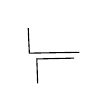
\begin{tikzpicture}[x=1em,y=1em,baseline]\draw (0,1.6)--(.04,.7)--(1.85,.73); \draw (1.66,.52)--(.31,.49)--(.34,-.39);\end{tikzpicture}} Le théorème est conséquence \deleted{\unsure{du théo|du théo.}}\inserted{de} cet \unsure{én$^{\mathrm{t}}$|én$^{\mathrm{cé}}$|est} équivalent

\unsure{à)|a')|a)|:)}

\uline{Théorème} $1'$ Soit $C$ une partie de $E$. Pour que $C$ soit convexe et fermé, il f. et s. que $C$ soit intersection de demi-espaces fermés.

Résulte du

\uline{Théorème $1''$} (Hahn-Banach) Soit $\deleted{\unsure{C}}U$ une partie \uline{convexe ouverte} de l'espace vectoriel \inserted{réel} $E$ de dim finie, $F\subsetneq E$ un sous-espace vectoriel de $E$ tel que $F\cap\deleted{\unsure{C}}U=\varnothing$, alors $\exists$ hyperplan $H$ de $E$ contenant $F$, tel que $H\cap U=\varnothing$.
